% MindBox — Complete Project Documentation (Hardware + Web Companion)
% Compile: pdflatex MindBox-Project-Documentation.tex (run twice for TOC)
% Recommended: TeX Live, MiKTeX, or Overleaf

\documentclass[11pt,a4paper]{report}

\usepackage[utf8]{inputenc}
\usepackage[T1]{fontenc}
\usepackage{lmodern}
\usepackage[margin=2.5cm]{geometry}
\usepackage{graphicx}
\usepackage{hyperref}
\usepackage{xcolor}
\usepackage{booktabs}
\usepackage{longtable}
\usepackage{enumitem}
\usepackage{listings}
\usepackage{array}
\usepackage{tikz}
\usetikzlibrary{arrows.meta, positioning, shapes.geometric, fit, backgrounds, calc}

\hypersetup{
  colorlinks=true,
  linkcolor=blue!70!black,
  urlcolor=blue!70!black,
  citecolor=blue!70!black,
  pdftitle={MindBox Project Documentation}
}

\definecolor{codebg}{RGB}{245,245,245}
\definecolor{keyword}{RGB}{0,80,160}
\definecolor{hwbg}{RGB}{255,248,240}
\definecolor{webbg}{RGB}{240,248,255}
\definecolor{notebg}{RGB}{248,248,220}

\lstset{
  basicstyle=\ttfamily\small,
  backgroundcolor=\color{codebg},
  frame=single,
  rulecolor=\color{gray!40},
  breaklines=true,
  columns=fullflexible,
  showstringspaces=false
}

\newcommand{\filepath}[1]{\texttt{#1}}
\newcommand{\keyword}[1]{\textbf{\textcolor{keyword}{#1}}}
\newcommand{\designbox}[2]{%
  \noindent\fcolorbox{blue!40}{webbg}{%
    \parbox{\dimexpr\linewidth-2\fboxsep-2\fboxrule}{%
      \textbf{Design decision:} #1\\[0.3em]#2}}%
  \vspace{0.6em}}

\title{%
  \textbf{MindBox --- Study Assistor}\\[0.6em]
  \large Complete Project Documentation\\[0.3em]
  \normalsize IoT Focus Device + Web Companion Application}
\author{Taiyo Yemin \and Maor Lisker \and Roy Avidan\\[0.4em]
\small ICST --- Interdisciplinary Center for Smart Technologies\\
Taub Faculty of Computer Science, Technion}
\date{June 2026}

\begin{document}
\maketitle

\begin{abstract}
\textbf{MindBox} is an IoT study-assistant system for university students. A desk-mounted
ESP32 device runs Pomodoro-style focus sessions, samples the local environment (noise,
light, temperature, presence), and coaches the user with haptics and optional adaptive
nudges---\emph{without requiring a phone during study}. A companion web application
(TanStack Start + React + Supabase) provides history, analytics, calendar planning,
exports, social features, and device pairing. This document describes the \emph{entire}
project: system vision, end-to-end architecture, \textbf{Arduino setup and wiring},
a full \textbf{metrics and heuristics} reference, and dedicated chapters for
\textbf{hardware firmware} and the \textbf{web application}. Firmware version
\filepath{0.2.0} at time of writing.
\end{abstract}

\tableofcontents
\listoffigures
\newpage

%==============================================================================
\chapter{Introduction}
%==============================================================================

\section{Problem and vision}

Students struggle to maintain consistent focus and rarely have objective data about
\emph{when} and \emph{where} they study best. MindBox combines a physical ritual (start
on the box, not on the phone) with environmental sensing and cloud-backed analytics.

\begin{itemize}[leftmargin=*]
  \item \textbf{On the desk:} timer, presence detection, coaching, offline persistence.
  \item \textbf{In the browser:} long-term memory, charts, insights, planning, exports.
  \item \textbf{Explicit disclaimer:} the \keyword{Focus Load Estimate} (FLE) is a
        transparent heuristic---never a clinical or validated measurement.
\end{itemize}

\section{Repository layout}

\begin{table}[h]
\centering
\caption{Main project folders (active code).}
\begin{tabular}{@{}ll@{}}
\toprule
\textbf{Path} & \textbf{Contents} \\
\midrule
\filepath{MindBox - hardware/MindBox/} & ESP32 firmware (Arduino/C++) \\
\filepath{mindbox-companion-forge-main/} & Web companion (TanStack Start + Supabase) \\
\filepath{Unit Tests/} & Isolated hardware validation sketches \\
\filepath{Documentation/} & Project documentation (this file) \\
\bottomrule
\end{tabular}
\end{table}

\section{User types}

\begin{description}[leftmargin=2.2cm, style=nextline]
  \item[Primary user] Person at the desk; interacts with encoder, button, OLED.
  \item[Observer] Roommates or family who may review exported summaries.
  \item[Analyst / admin] User reviewing trends in the web app; optional reviewer role.
\end{description}

%==============================================================================
\chapter{System architecture (overview)}
%==============================================================================

\section{Two-layer product split}

\designbox{Offline-first, cloud-enhanced}{The box must work without connectivity.
Sessions, coaching, and OLED UX never block on HTTP. Cloud sync is additive: save
locally, upload when Wi-Fi is available, analyse in the web app.}

\begin{figure}[h]
\centering
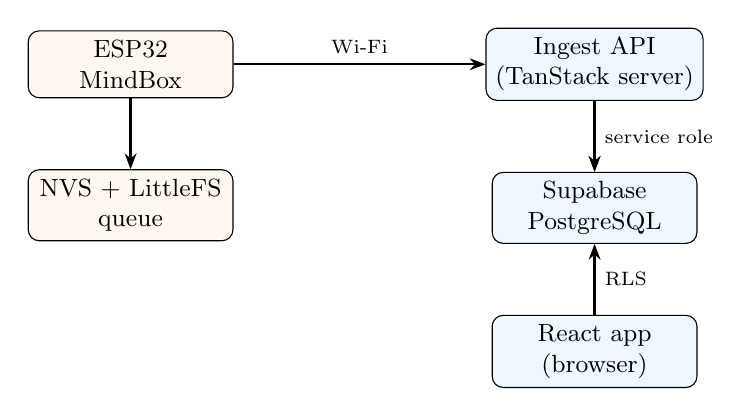
\begin{tikzpicture}[
  node distance=0.9cm and 1.2cm,
  box/.style={draw, rounded corners, minimum width=2.6cm, minimum height=0.85cm, align=center, font=\small},
  arr/.style={-{Stealth[length=2mm]}, thick}
]
  \node[box, fill=hwbg] (esp) {ESP32\\MindBox};
  \node[box, fill=hwbg, below=of esp] (nvs) {NVS + LittleFS\\queue};
  \node[box, fill=webbg, right=3.2cm of esp] (ingest) {Ingest API\\(TanStack server)};
  \node[box, fill=webbg, below=of ingest] (db) {Supabase\\PostgreSQL};
  \node[box, fill=webbg, below=of db] (web) {React app\\(browser)};

  \draw[arr] (esp) -- node[above, font=\scriptsize]{Wi-Fi} (ingest);
  \draw[arr] (esp) -- (nvs);
  \draw[arr] (ingest) -- (db);
  \draw[arr] (web) -- node[right, font=\scriptsize]{RLS} (db);
  \draw[arr] (ingest) -- node[right, font=\scriptsize]{service role} (db);
\end{tikzpicture}
\caption{End-to-end data flow. Device $\rightarrow$ ingest $\rightarrow$ database; browser $\rightarrow$ Supabase with row-level security.}
\end{figure}

\section{Shared contracts}

Firmware (\filepath{focus\_load.h}, \filepath{Payload.cpp}), the TypeScript module
\filepath{src/lib/focus-load.ts}, Zod schemas in \filepath{ingest.server.ts}, and the
device simulator all share the same session JSON shape and FLE formula. This prevents
``the app shows different numbers than the box.''

\section{Focus Load Estimate (FLE)}

\begin{lstlisting}
FLE = round(100 * (
  0.3 * (elapsed / target) +
  0.3 * normalizedNoise +
  0.2 * ambientLightVariance +
  0.2 * (presenceInterruptions / 5)
))
\end{lstlisting}

Each term is clamped to $[0,1]$ before weighting. Weights sum to $1.0$.
Chapter~\ref{ch:metrics} gives the full metrics catalog and design rationale.

%==============================================================================
\part{Hardware --- ESP32 firmware}
%==============================================================================

\chapter{Hardware platform and components}

\section{Microcontroller}

\begin{itemize}[leftmargin=*]
  \item \textbf{Board:} DOIT ESP32 DevKit V1 (\filepath{esp32doit-devkit-v1})
  \item \textbf{Entry point:} \filepath{MindBox.ino} (thin orchestrator; logic in modules)
  \item \textbf{Firmware version:} \filepath{FW\_VERSION = "0.2.0"}
  \item \textbf{Serial diagnostics:} 115200 baud
\end{itemize}

\section{Bill of materials (wired / active)}

\begin{longtable}{@{}p{3.2cm}p{4.2cm}p{6.8cm}@{}}
\toprule
\textbf{Component} & \textbf{Interface} & \textbf{Role} \\
\midrule
\endhead
KY-040 rotary encoder & GPIO 18, 19, 23 & Menu navigation (cursor + select) \\
6$\times$6 tact button & GPIO 4 & Side button: pause, abort, menu select \\
OLED 128$\times$64 & I2C (SDA 21, SCL 22) & Timer, menus, diagnostics (SH1106/SSD1306 auto-detect) \\
GY-MAX9814 microphone & ADC GPIO 34 & Ambient noise (normalized 0--1) \\
VL53L1X ToF sensor & I2C 0x29 & Desk presence (distance mm) \\
DHT11 & GPIO 26 & Temperature (humidity available on chip, not uploaded) \\
Keyes KY-018 & ADC GPIO 35 & Light level + variance for FLE \\
Coin vibration motor & GPIO 25 (NPN/MOSFET) & Haptic patterns (non-blocking) \\
\midrule
\multicolumn{3}{l}{\textit{Planned / stubbed: WS2812B LED ring (GPIO 5), LiPo battery (GPIO 36), BLE, SPDT toggle (GPIO 32)}} \\
\bottomrule
\caption{Hardware components and pin assignments (\filepath{config.h}).}
\end{longtable}

\section{Wiring summary}

\begin{table}[h]
\centering
\caption{GPIO pin map (single source of truth: \filepath{config.h}).}
\begin{tabular}{@{}lll@{}}
\toprule
\textbf{GPIO} & \textbf{Function} & \textbf{Notes} \\
\midrule
4  & Side button & \texttt{INPUT\_PULLUP}, active low \\
5  & LED ring data & Stub; needs 5\,V + 470\,$\Omega$ + 1000\,$\mu$F \\
18, 19, 23 & Encoder CLK, DT, SW & Shaft click unused \\
21, 22 & I2C SDA, SCL & OLED + ToF; 100\,kHz \\
25 & Haptic driver & Avoid GPIO 2 (onboard LED conflict) \\
26 & DHT11 DATA & 3.3\,V; 4.7--10\,k$\Omega$ pull-up \\
32 & SPDT toggle & Optional Work/Break switch \\
34 & Microphone OUT & ADC1 input-only \\
35 & KY-018 AO & ADC1; reserved for light \\
36 & Battery ADC & Reserved when \texttt{HAS\_BATTERY=1} \\
\bottomrule
\end{tabular}
\end{table}

%------------------------------------------------------------------------------
\chapter{Wiring guide --- what connects to what}
\label{ch:wiring}
%------------------------------------------------------------------------------

\section{Power and ground rules}

\begin{itemize}[leftmargin=*]
  \item Use the ESP32 \textbf{3V3} pin for all sensor modules (not 5\,V on GPIO signals).
  \item Tie all module \textbf{GND} legs to a common ground rail on the breadboard.
  \item Keep I2C wires (SDA/SCL) short; both OLED and VL53L1X share the same bus.
  \item The vibration motor uses a \textbf{transistor} (NPN or MOSFET): GPIO\,25 drives the
        base/gate; motor power may come from 5\,V; do \textbf{not} connect the motor directly
        to a GPIO pin.
  \item Do \textbf{not} use GPIO\,2 for the motor --- it shares the onboard blue LED on the
        DOIT DevKit V1 and drives weakly.
\end{itemize}

\section{Per-component connections}

\begin{longtable}{@{}p{2.6cm}p{3.8cm}p{6.8cm}@{}}
\toprule
\textbf{Component} & \textbf{Pins on module} & \textbf{Connect to ESP32} \\
\midrule
\endhead
OLED 128$\times$64 &
VCC, GND, SDA, SCL &
3V3, GND, GPIO\,21 (SDA), GPIO\,22 (SCL) \\
VL53L1X ToF &
VCC, GND, SDA, SCL &
3V3, GND, GPIO\,21, GPIO\,22 (I2C addr.\ 0x29) \\
KY-040 encoder &
+, GND, CLK, DT, SW (optional) &
3V3, GND, GPIO\,18 (CLK), GPIO\,19 (DT), GPIO\,23 (SW) \\
Side button (6$\times$6) &
Two diagonal legs &
GPIO\,4 $\leftrightarrow$ one leg; other leg $\rightarrow$ GND \\
GY-MAX9814 mic &
VCC, GND, OUT &
3V3, GND, GPIO\,34 (ADC, input-only) \\
DHT11 &
VCC, DATA, GND &
3V3, GPIO\,26 (DATA), GND; add 4.7--10\,k$\Omega$ DATA$\rightarrow$3V3 if missing \\
Keyes KY-018 &
VCC, GND, AO, DO &
3V3, GND, GPIO\,35 (AO only); leave DO unconnected \\
Haptic motor &
Via driver circuit &
GPIO\,25 $\rightarrow$ transistor base; motor + flyback diode per driver datasheet \\
\bottomrule
\caption{Detailed wiring: module pin $\rightarrow$ ESP32 pin.}
\end{longtable}

\section{Wiring diagram (logical)}

\begin{figure}[h]
\centering
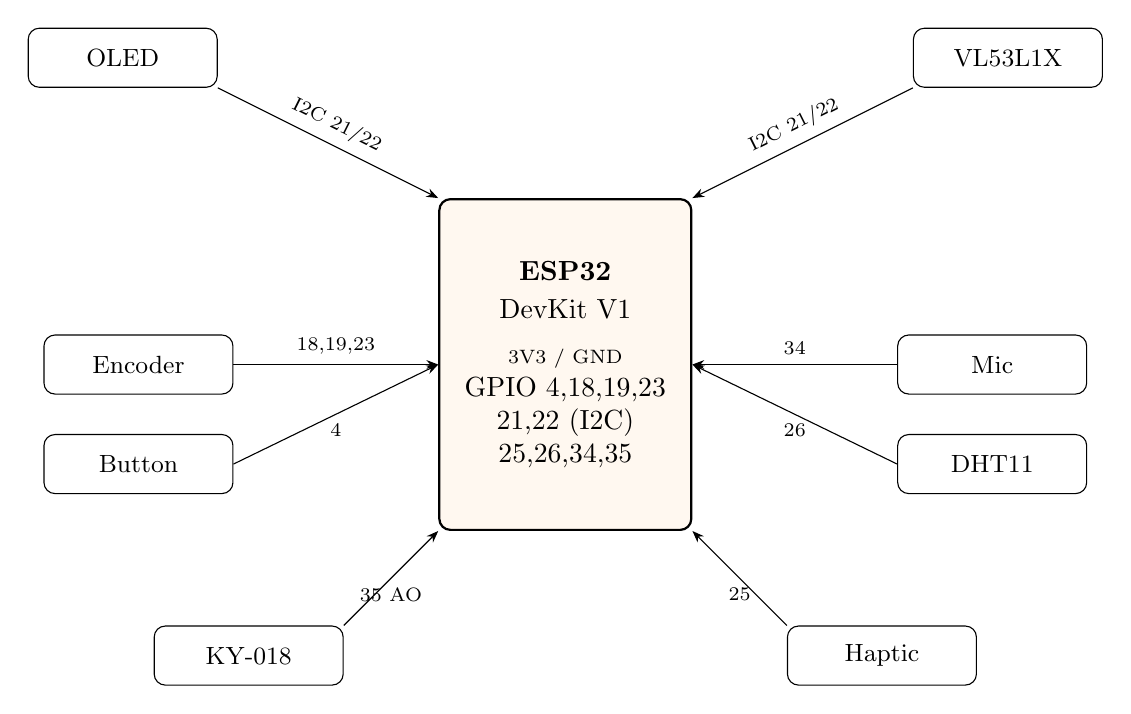
\begin{tikzpicture}[
  esp/.style={draw, thick, rounded corners, minimum width=3.2cm, minimum height=4.2cm, align=center, fill=hwbg},
  mod/.style={draw, rounded corners, minimum width=2.4cm, minimum height=0.75cm, align=center, font=\small},
  arr/.style={-{Stealth[length=1.5mm]}, font=\scriptsize}
]
  \node[esp] (esp32) at (0,0) {\textbf{ESP32}\\[2pt]DevKit V1\\[4pt]
    \scriptsize 3V3 / GND\\GPIO 4,18,19,23\\21,22 (I2C)\\25,26,34,35};

  \node[mod, above left=1.4cm and 2.8cm of esp32] (oled) {OLED};
  \node[mod, above right=1.4cm and 2.8cm of esp32] (tof) {VL53L1X};
  \node[mod, left=2.6cm of esp32] (enc) {Encoder};
  \node[mod, left=2.6cm, below=0.5cm of enc] (btn) {Button};
  \node[mod, right=2.6cm of esp32] (mic) {Mic};
  \node[mod, right=2.6cm, below=0.5cm of mic] (dht) {DHT11};
  \node[mod, below left=1.2cm and 1.2cm of esp32] (light) {KY-018};
  \node[mod, below right=1.2cm and 1.2cm of esp32] (hap) {Haptic};

  \draw[arr] (oled.south east) -- node[above, sloped]{I2C 21/22} (esp32.north west);
  \draw[arr] (tof.south west) -- node[above, sloped]{I2C 21/22} (esp32.north east);
  \draw[arr] (enc.east) -- node[above]{18,19,23} (esp32.west);
  \draw[arr] (btn.east) -- node[below]{4} (esp32.west);
  \draw[arr] (mic.west) -- node[above]{34} (esp32.east);
  \draw[arr] (dht.west) -- node[below]{26} (esp32.east);
  \draw[arr] (light.north east) -- node[below]{35 AO} (esp32.south west);
  \draw[arr] (hap.north west) -- node[below]{25} (esp32.south east);
\end{tikzpicture}
\caption{Logical wiring overview. All modules also share 3V3 and GND with the ESP32.}
\label{fig:wiring}
\end{figure}

\section{Recommended bring-up order}

\begin{enumerate}[leftmargin=*]
  \item Wire power only; flash a blank sketch; confirm USB serial at 115200.
  \item Run unit-test sketches in \filepath{Unit Tests/} (button, encoder, mic, lazer, dht11, light) one at a time.
  \item Wire I2C bus; confirm OLED and ToF in serial I2C scan (addresses \texttt{0x3C}/\texttt{0x3D} and \texttt{0x29}).
  \item Flash full \filepath{MindBox.ino}; verify boot self-test lists all sensors \texttt{ok}.
  \item Provision Wi-Fi (serial \texttt{w}); pair device in web app; run a short session and check \texttt{/history}.
\end{enumerate}

%------------------------------------------------------------------------------
\chapter{Arduino IDE setup and flashing}
\label{ch:arduino}
%------------------------------------------------------------------------------

\section{Tools}

You may use \textbf{Arduino IDE 2.x} or \textbf{VS Code / Cursor} with the Arduino extension.
Project settings live in \filepath{.vscode/arduino.json}:
\begin{lstlisting}
board: esp32:esp32:esp32doit-devkit-v1
sketch: MindBox - hardware/MindBox/MindBox.ino
upload speed: 921600
\end{lstlisting}
Change the \texttt{port} field to your COM port (Windows) or \texttt{/dev/ttyUSB0} (Linux).

\section{Install ESP32 board support}

\begin{enumerate}[leftmargin=*]
  \item Arduino IDE $\rightarrow$ \textbf{File $\rightarrow$ Preferences $\rightarrow$ Additional Board Manager URLs}:
\begin{lstlisting}
https://raw.githubusercontent.com/espressif/arduino-esp32/gh-pages/package_esp32_index.json
\end{lstlisting}
  \item \textbf{Tools $\rightarrow$ Board $\rightarrow$ Boards Manager} $\rightarrow$ install \textbf{esp32} by Espressif (2.x).
  \item Select board: \textbf{DOIT ESP32 DEVKIT V1} (or \texttt{esp32doit-devkit-v1}).
\end{enumerate}

\section{Partition scheme (required for upload queue)}

The firmware stores pending session JSON on \textbf{LittleFS}. In Arduino IDE:
\textbf{Tools $\rightarrow$ Partition Scheme} $\rightarrow$ choose a scheme that includes
SPIFFS or LittleFS (e.g.\ ``Default 4MB with spiffs'' or project-specific LittleFS layout).
Without filesystem partition, \texttt{UploadQueue} cannot persist sessions offline.

\section{Install libraries}

Via \textbf{Sketch $\rightarrow$ Include Library $\rightarrow$ Manage Libraries}:

\begin{table}[h]
\centering
\caption{Required Arduino libraries.}
\begin{tabular}{@{}ll@{}}
\toprule
\textbf{Library} & \textbf{Purpose} \\
\midrule
Adafruit BusIO & I2C helpers \\
Adafruit GFX Library & OLED drawing \\
Adafruit SH110X & SH1106 OLED driver \\
Adafruit SSD1306 & SSD1306 OLED driver \\
Adafruit VL53L1X & ToF presence sensor \\
DHT sensor library (Adafruit) & DHT11 temperature \\
Adafruit Unified Sensor & DHT dependency \\
AiEsp32RotaryEncoder & KY-040 encoder \\
\bottomrule
\end{tabular}
\end{table}

\section{Optional compile-time secrets}

Create \filepath{MindBox - hardware/MindBox/SECRETS.h} (gitignored) to bake in Wi-Fi and cloud
defaults, \emph{or} leave empty and provision later via serial \texttt{w}:
\begin{lstlisting}
#define SECRET_WIFI_SSID     "your-ssid"
#define SECRET_WIFI_PASS     "your-password"
#define SECRET_APP_BASE_URL  "http://192.168.1.x:8080"
#define SECRET_DEVICE_SECRET "long-random-string"
\end{lstlisting}
The device secret must match \texttt{DEVICE\_INGEST\_SECRET} in the web app \filepath{.env}.

\section{Upload and verify}

\begin{enumerate}[leftmargin=*]
  \item Connect ESP32 via USB; select the correct port under \textbf{Tools $\rightarrow$ Port}.
  \item Open \filepath{MindBox - hardware/MindBox/MindBox.ino}; click \textbf{Upload}.
  \item Open \textbf{Serial Monitor}: baud \textbf{115200}, line ending \textbf{Newline}.
  \item Expect \texttt{==== MindBox self-test ====} with OLED, ToF, mic, light, temp lines.
  \item Press \texttt{h} for help; \texttt{m} for live monitor; \texttt{c} for sensor calibration.
\end{enumerate}

\section{Troubleshooting}

\begin{table}[h]
\centering
\caption{Common hardware bring-up issues.}
\begin{tabular}{@{}p{4cm}p{8.8cm}@{}}
\toprule
\textbf{Symptom} & \textbf{Likely fix} \\
\midrule
I2C scan empty & Check SDA=21, SCL=22, 3V3, GND; reduce wire length \\
OLED not found & Try both SH1106/SSD1306 auto-detect; verify I2C address \\
DHT reads \texttt{nan} & GPIO\,26 only; add pull-up; wait 2\,s between reads \\
Button stuck LOW & Use \textbf{diagonal} tact pins; GPIO\,4 to one leg, GND to other \\
Upload fails & Hold BOOT button during flash; try lower upload speed \\
No Wi-Fi / cloud & Serial \texttt{w}; match URL and \texttt{x-device-secret} to server \\
\bottomrule
\end{tabular}
\end{table}

\chapter{Firmware architecture}

\section{Design principles}

\begin{enumerate}[leftmargin=*]
  \item \textbf{Single-responsibility modules} --- one \filepath{.h} + one \filepath{.cpp} per concern.
  \item \textbf{Acyclic dependencies} --- \filepath{Display} driven by \texttt{UiModel} only; no cycles.
  \item \textbf{One config file} --- \filepath{config.h} for pins, flags, tunables.
  \item \textbf{Offline-first sync} --- NVS compact log + LittleFS upload queue.
\end{enumerate}

\section{Module map}

\begin{longtable}{@{}p{2.4cm}p{5.2cm}p{5.8cm}@{}}
\toprule
\textbf{Module} & \textbf{Responsibility} & \textbf{Key interactions} \\
\midrule
\endhead
\texttt{MindBox.ino} & \texttt{setup()} / \texttt{loop()} wiring & Ticks all modules \\
\texttt{StateMachine} & Session lifecycle FSM & Orchestrates menu, session, cloud \\
\texttt{Menu} & Pointer menus on OLED & Inputs, Display, Storage \\
\texttt{Session} & Countdown, sampling, FLE & Sensors, \texttt{esp\_timer} clock \\
\texttt{Sensors} & Mic, ToF, DHT11, KY-018 & NVS calibration scales \\
\texttt{Storage} & NVS persistence & Config, checkpoint, session log \\
\texttt{UploadQueue} & LittleFS session backlog & Full JSON payloads \\
\texttt{Cloud} & Wi-Fi, NTP, HTTP ingest & Upload drain, config pull \\
\texttt{Payload} & \texttt{sessionJson()} serializer & Matches web Zod schema \\
\texttt{Display} & OLED screens & \texttt{UiModel} only \\
\texttt{Haptics} & Vibration patterns & Non-blocking state machine \\
\texttt{Inputs} & Encoder + button & Debounce, long-press \\
\texttt{Diagnostics} & Serial monitor & Self-test, calibration commands \\
\texttt{focus\_load.h} & FLE heuristic & Mirror of \filepath{focus-load.ts} \\
\bottomrule
\caption{Firmware module responsibilities.}
\end{longtable}

\section{Dependency graph}

\begin{figure}[h]
\centering
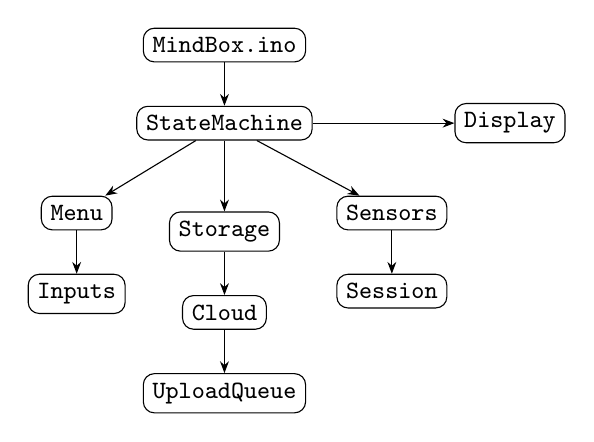
\begin{tikzpicture}[
  node distance=0.55cm and 0.9cm,
  mod/.style={draw, rounded corners, font=\small\ttfamily, align=center},
  arr/.style={-{Stealth[length=1.5mm]}}
]
  \node[mod] (ino) {MindBox.ino};
  \node[mod, below=of ino] (sm) {StateMachine};
  \node[mod, below left=0.7cm and 0.3cm of sm] (menu) {Menu};
  \node[mod, below=of menu] (inputs) {Inputs};
  \node[mod, below right=0.7cm and 0.3cm of sm] (sens) {Sensors};
  \node[mod, below=of sens] (sess) {Session};
  \node[mod, right=1.8cm of sm] (disp) {Display};
  \node[mod, below=0.9cm of sm] (stor) {Storage};
  \node[mod, below=of stor] (cloud) {Cloud};
  \node[mod, below=of cloud] (uq) {UploadQueue};

  \draw[arr] (ino) -- (sm);
  \draw[arr] (sm) -- (menu);
  \draw[arr] (menu) -- (inputs);
  \draw[arr] (sm) -- (sens);
  \draw[arr] (sens) -- (sess);
  \draw[arr] (sm) -- (disp);
  \draw[arr] (sm) -- (stor);
  \draw[arr] (stor) -- (cloud);
  \draw[arr] (cloud) -- (uq);
\end{tikzpicture}
\caption{Firmware dependency direction (no cycles).}
\end{figure}

\chapter{Session lifecycle and user interface}

\section{State machine}

\begin{lstlisting}
BOOTING -> IDLE
IDLE    -> RUNNING | PAIRING | DIAG
RUNNING -> PAUSED | COMPLETE | ERROR | IDLE (abort)
PAUSED  -> RUNNING | IDLE (end)
COMPLETE-> LOGGING -> IDLE
\end{lstlisting}

\section{Pointer menu (idle)}

Rotate encoder = move cursor; side button short = select; long = back.
During \texttt{RUNNING}: short = pause, long = abort.

\begin{lstlisting}
> Start
  Mode            WORK
  Duration        25 min
  Settings
  Device          (Pair, Diagnostics)
  About
\end{lstlisting}

\section{Adaptive coaching}

When \texttt{adaptiveCoaching} is enabled and FLE exceeds 75 during WORK:
\begin{itemize}[leftmargin=*]
  \item Optional OLED nudge: ``Consider a break''
  \item Optional haptic pattern (5\,min cooldown)
  \item Optional auto-pause (\texttt{PAUSE\_COACHING})
\end{itemize}

\section{Presence-based pause}

VL53L1X distance $\leq$ 700\,mm $\Rightarrow$ present. Absent for 30\,s $\Rightarrow$ pause
(\texttt{PAUSE\_AWAY}). Absent for 5\,min $\Rightarrow$ auto-end (interrupted).

\chapter{Sensors and environment sampling}

\section{Sampling policy}

\begin{table}[h]
\centering
\caption{Environment sample intervals (\filepath{Session.cpp} + \filepath{StateMachine.cpp}).}
\begin{tabular}{@{}ll@{}}
\toprule
\textbf{Condition} & \textbf{Interval} \\
\midrule
WORK, coaching off & 60\,s \\
WORK, adaptive coaching on & 30\,s \\
BREAK & 120\,s \\
PAUSED & Off (no \texttt{Session::tick}) \\
\bottomrule
\end{tabular}
\end{table}

Each sample records: elapsed time, FLE, noise, temperature, light lux. Aggregates at
session end feed \texttt{env} and \texttt{envSamples} in the upload JSON.

\section{NVS field calibration}

Mic, light, and temperature scales are stored in NVS and adjustable without reflash.
Serial command \textbf{c} at 115200 baud:

\begin{table}[h]
\centering
\begin{tabular}{@{}ll@{}}
\toprule
\textbf{Command} & \textbf{Effect} \\
\midrule
\texttt{c} & Print scales + live readings \\
\texttt{c noise 1800} & Mic ADC peak-to-peak $\rightarrow$ 1.0 normalized \\
\texttt{c light 1200} & KY-018 ADC $\rightarrow$ lux estimate scale \\
\texttt{c lightvar 2000} & Light flicker $\rightarrow$ FLE variance scale \\
\texttt{c temp -1.5} & DHT11 temperature offset (\textdegree C) \\
\texttt{c reset} & Restore factory defaults \\
\bottomrule
\end{tabular}
\end{table}

\section{Sensor wiring notes}

\begin{itemize}[leftmargin=*]
  \item \textbf{DHT11:} 3.3\,V only; min 2\,s between reads; do not use input-only GPIO.
  \item \textbf{KY-018:} Use \textbf{AO} (analog); blue potentiometer affects DO only.
  \item \textbf{Microphone:} Rolling 1\,Hz peak-to-peak window; scale via NVS.
\end{itemize}

\chapter{Persistence, sync, and checkpoints}

\section{Storage layers}

\begin{description}[leftmargin=2.8cm, style=nextline]
  \item[NVS \texttt{slog}] Ring of 16 compact session log entries for on-device history.
  \item[NVS checkpoint v3] In-progress session: timer, set progress, last 10 samples + noise aggregates.
  \item[LittleFS upload queue] Up to 12 full session JSON blobs; drop-oldest on overflow.
\end{description}

\designbox{Never block a session on HTTP}{Telemetry and upload run in \texttt{Cloud::tick()}
outside active countdown-critical paths where possible. Session clock uses
\texttt{esp\_timer} at 10\,ms so main-loop stalls do not skip time.}

\section{Checkpoint sample tail}

On pause, start, end, or power loss, checkpoint v3 saves:
\begin{itemize}[leftmargin=*]
  \item Last \texttt{CHECKPOINT\_TAIL\_MAX} (=10) \texttt{Sample} records
  \item \texttt{noiseSum}, \texttt{noisePeak}, \texttt{noiseN} for correct session averages
  \item Cold-boot resume calls \texttt{Session::alignSampleTimer()} (millis resets)
\end{itemize}

Samples older than the tail are not recovered---minimal NVS footprint by design.

\section{Cloud HTTP endpoints (device)}

\begin{table}[h]
\centering
\begin{tabular}{@{}lll@{}}
\toprule
\textbf{Method} & \textbf{Path} & \textbf{Purpose} \\
\midrule
POST & \texttt{/ingest/sessions} & Batch session upload (idempotent) \\
POST & \texttt{/ingest/telemetry} & Heartbeat + sensor health \\
POST & \texttt{/ingest/pairing} & Publish 6-digit pairing code \\
GET  & \texttt{/ingest/config?deviceId=} & Settings downlink \\
\bottomrule
\end{tabular}
\end{table}

Header: \texttt{x-device-secret}. Provisioning: serial \texttt{w} command stores SSID, password, base URL, secret in NVS.

\section{Arduino libraries}

\begin{itemize}[leftmargin=*]
  \item Adafruit BusIO, GFX, SH110X, SSD1306
  \item Adafruit VL53L1X (ToF presence)
  \item DHT sensor library (Adafruit) + Adafruit Unified Sensor
  \item AiEsp32RotaryEncoder (encoder)
  \item Preferences (NVS), LittleFS (upload queue)
\end{itemize}

\chapter{Hardware diagnostics and testing}

\section{Serial commands}

\begin{tabular}{@{}ll@{}}
\toprule
\textbf{Key} & \textbf{Action} \\
\midrule
\texttt{m} & Toggle 1\,Hz live monitor \\
\texttt{c} & Calibration (see above) \\
\texttt{b} & Button wiring test (8\,s) \\
\texttt{w} & Wi-Fi / cloud provisioning \\
\texttt{q} & Upload queue status \\
\texttt{d} & Single diagnostic dump \\
\texttt{h} & Help \\
\bottomrule
\end{tabular}

\section{Unit test sketches}

Folder \filepath{Unit Tests/} contains isolated \filepath{.ino} files for button, encoder,
microphone, laser (ToF), vibration, and dedicated \filepath{dht11/}, \filepath{light\_ky018/}
when present. Run each sketch alone before integrating into MindBox.

\section{Implementation status (hardware)}

\begin{table}[h]
\centering
\begin{tabular}{@{}ll@{}}
\toprule
\textbf{Feature} & \textbf{Status} \\
\midrule
Encoder, button, OLED, haptics & Active \\
Microphone, ToF presence & Active \\
DHT11, KY-018 light & Active \\
NVS calibration, adaptive sampling & Active \\
Checkpoint sample tail (v3) & Active \\
Wi-Fi, upload queue, ingest & Active \\
LED ring, battery, BLE & Stubbed \\
Captive portal Wi-Fi setup & Planned (serial \texttt{w} today) \\
TLS on device (\texttt{CLOUD\_USE\_TLS}) & Off by default (dev) \\
\bottomrule
\end{tabular}
\end{table}

%==============================================================================
\part{Web application --- MindBox Companion}
%==============================================================================

\chapter{Web stack and project structure}

\section{Technology choices}

\begin{table}[h]
\centering
\caption{Web companion technology stack.}
\begin{tabular}{@{}ll@{}}
\toprule
\textbf{Layer} & \textbf{Technology} \\
\midrule
Framework & TanStack Start + React 19 \\
Routing & TanStack Router (file-based, \filepath{src/routes/}) \\
Data fetching & TanStack Query \\
Styling & Tailwind CSS 4, Radix UI (shadcn-style) \\
Build & Vite 7, Nitro 3 \\
Database & Supabase (PostgreSQL + Auth + RLS) \\
Validation & Zod (ingest + forms) \\
Tests & Vitest (pure logic modules) \\
Deploy target & Cloudflare Workers (via Lovable/Nitro config) \\
\bottomrule
\end{tabular}
\end{table}

\section{Repository layout (web)}

\begin{lstlisting}
mindbox-companion-forge-main/
  src/
    routes/           # File-based pages
    lib/
      focus-load.ts   # FLE + SessionPayload contract
      ingest/         # Device ingest handlers
      queries/        # React Query hooks
      api/            # Server functions
    components/       # UI (AppShell, charts, cards)
    server.ts         # Ingest route interception
  supabase/migrations/  # 0001--0010 SQL schema
  scripts/
    simulator.ts      # Fake device for dev
    cleanup-simulator.ts
\end{lstlisting}

\designbox{Device is source of truth for sessions}{The web app does not start or stop
focus timers. Users begin and end sessions on the box. The app's role is memory,
analysis, configuration downlink, and pairing---not remote control of the clock.}

\chapter{Application features and routes}

\section{Primary routes}

\begin{longtable}{@{}p{2.8cm}p{9.8cm}@{}}
\toprule
\textbf{Route} & \textbf{Purpose} \\
\midrule
\endhead
\texttt{/} & Dashboard: today/week focus, streaks, quick stats \\
\texttt{/history} & Session list with filters \\
\texttt{/session/:id} & Session detail: FLE chart, env samples, metadata \\
\texttt{/insights} & Patterns, correlations, wellbeing estimates \\
\texttt{/calendar} & Schedule: classes, exams, recovery balance \\
\texttt{/device} & Pairing (6-digit code), status, BLE beta \\
\texttt{/settings} & User preferences, coaching toggles, goals \\
\texttt{/exports} & CSV / PDF report generation \\
\texttt{/friends} & Social graph, friend notifications \\
\texttt{/leaderboard} & Focus leaderboard among friends \\
\texttt{/reviewers} & Read-only reviewer access grants \\
\texttt{/simulator} & Dev UI for simulator scenarios \\
\texttt{/login} & Google OAuth via Supabase \\
\bottomrule
\caption{Web application routes.}
\end{longtable}

\section{Key feature areas}

\begin{itemize}[leftmargin=*]
  \item \textbf{Focus history} --- chronological sessions with mode, duration, status, FLE.
  \item \textbf{Environmental insights} --- noise, temperature, light vs.\ focus score.
  \item \textbf{Wellbeing estimates} --- heuristic recovery balance (not clinical).
  \item \textbf{External load} --- lectures/labs feed recovery planning (migration 0006).
  \item \textbf{Streaks and goals} --- daily focus targets and gamification.
  \item \textbf{Email reports} --- PDF via PDFKit / Puppeteer (server-side).
  \item \textbf{Reviewer access} --- mentors see scoped student data (read-only RLS).
\end{itemize}

\chapter{Backend: Supabase and ingest API}

\section{Database schema (core tables)}

\begin{longtable}{@{}p{3.4cm}p{9.2cm}@{}}
\toprule
\textbf{Table} & \textbf{Purpose} \\
\midrule
\endhead
\texttt{profiles} & App user mirror of \texttt{auth.users} \\
\texttt{devices} & Physical MindBox units (\texttt{id} = hardware device id) \\
\texttt{device\_profiles} & Multi-user slots per device (Story 7) \\
\texttt{device\_pairing\_codes} & 6-digit claim codes \\
\texttt{device\_status} & Latest telemetry per device \\
\texttt{sessions} & Focus session summaries; unique \texttt{(device\_id, id)} \\
\texttt{focus\_load\_samples} & Per-minute FLE time series \\
\texttt{env\_samples} & Per-minute noise/temp/light \\
\texttt{user\_settings} & Coaching, quiet hours, device show-timer (0010) \\
\texttt{friendships}, \texttt{reviewer\_grants} & Social and mentor access \\
\texttt{schedule\_events} & Calendar entries (0007--0009) \\
\bottomrule
\caption{Primary Supabase tables.}
\end{longtable}

\section{Row-level security}

Authenticated users access their own sessions via \texttt{user\_id}. Reviewers receive
scoped \texttt{SELECT} through grant policies. Device ingest uses the \textbf{service
role} server-side only---never exposed to the browser.

\section{Ingest endpoints}

Implemented in \filepath{src/lib/ingest/ingest.server.ts}, routed via \filepath{server.ts}:

\begin{enumerate}[leftmargin=*]
  \item \textbf{POST /ingest/sessions} --- Zod-validated batch; upsert on
        \texttt{(device\_id, session\_id)}; resolves \texttt{user\_id} from device ownership
        and profile slot.
  \item \textbf{POST /ingest/telemetry} --- Updates \texttt{device\_status}.
  \item \textbf{POST /ingest/pairing} --- Stores pairing code for app claim flow.
  \item \textbf{GET /ingest/config} --- Returns merged user/device settings for downlink.
\end{enumerate}

Authorization: constant-time compare of \texttt{x-device-secret} header.

\section{Migrations}

Apply \filepath{supabase/migrations/0001\_init.sql} through \filepath{0010\_device\_config.sql}
in order in the Supabase SQL Editor, then run:
\begin{lstlisting}
NOTIFY pgrst, 'reload schema';
\end{lstlisting}

\chapter{Shared logic and testing}

\section{\filepath{focus-load.ts}}

Single source for:
\begin{itemize}[leftmargin=*]
  \item \texttt{computeFocusLoad()} --- same formula as firmware
  \item \texttt{SessionPayload}, \texttt{TelemetryPayload} TypeScript interfaces
  \item Labels and caps (\texttt{PRESENCE\_INTERRUPTION\_CAP = 5})
\end{itemize}

\section{Vitest unit tests}

\filepath{npm run test} runs logic-only tests (no full Vite SSR stack):
\begin{itemize}[leftmargin=*]
  \item \filepath{focus-load.test.ts}, \filepath{insights.test.ts}, \filepath{wellbeing.test.ts}
  \item \filepath{streak.test.ts}, \filepath{schedule.test.ts}, \filepath{export.test.ts}
  \item \filepath{session-scope.test.ts}, \filepath{sensor-health.test.ts}, and others
\end{itemize}

\section{Device simulator}

\filepath{scripts/simulator.ts} POSTs to \texttt{/ingest/*} with deterministic session IDs
(idempotent re-runs). Scenarios: \texttt{--offline-then-sync}, \texttt{--low-battery},
\texttt{--sensor-fault}. Requires \texttt{npm run dev} and \texttt{DEVICE\_INGEST\_SECRET} in \filepath{.env}.

\chapter{Web setup and deployment}

\section{Local development}

\begin{enumerate}[leftmargin=*]
  \item \texttt{cd mindbox-companion-forge-main \&\& npm install}
  \item Copy \filepath{.env.example} $\rightarrow$ \filepath{.env} (Supabase URL, anon key, service role, ingest secret)
  \item Apply migrations 0001--0010 in Supabase SQL Editor
  \item Enable Google OAuth provider; add redirect URLs
  \item \texttt{npm run dev} $\rightarrow$ \texttt{http://localhost:8080}
\end{enumerate}

\section{Environment variables (essential)}

\begin{itemize}[leftmargin=*]
  \item \texttt{VITE\_SUPABASE\_URL}, \texttt{VITE\_SUPABASE\_ANON\_KEY}
  \item \texttt{SUPABASE\_SERVICE\_ROLE\_KEY} (server only)
  \item \texttt{DEVICE\_INGEST\_SECRET} (must match device NVS secret)
  \item \texttt{APP\_BASE\_URL} (device provisioning + callbacks)
\end{itemize}

\section{Implementation status (web)}

\begin{table}[h]
\centering
\begin{tabular}{@{}ll@{}}
\toprule
\textbf{Area} & \textbf{Status} \\
\midrule
Auth (Google), dashboard, history & Complete \\
Session detail charts, insights & Complete \\
Calendar, external load, exports & Complete \\
Friends, leaderboard, reviewers & Complete \\
Ingest API + simulator & Complete \\
Web Bluetooth (beta UI) & UI present; firmware BLE stubbed \\
CI/CD pipeline & Not configured in repo \\
\bottomrule
\end{tabular}
\end{table}

%==============================================================================
\part{Metrics, heuristics, and rationale}
%==============================================================================

\chapter{Metrics catalog}
\label{ch:metrics}

\section{Design principle: estimates, not diagnoses}

All derived scores in MindBox are \textbf{transparent heuristics}---useful patterns for
self-reflection, not clinical or validated measurements. The UI labels the Focus Load
Estimate (FLE) and wellbeing signals accordingly. Source of truth:
\filepath{focus-load.ts}, \filepath{wellbeing.ts}, \filepath{insights.ts},
\filepath{focus\_load.h} (firmware mirror).

\section{Session payload fields}

\begin{longtable}{@{}p{3.4cm}p{9.2cm}@{}}
\toprule
\textbf{Field} & \textbf{Meaning} \\
\midrule
\endhead
\texttt{deviceId} & Stable hardware ID (MAC-derived prefix) \\
\texttt{profileId} & Active user slot on shared device \\
\texttt{sessionId} & UUID; idempotency key with \texttt{deviceId} \\
\texttt{startedAt}, \texttt{endedAt} & ISO-8601 timestamps \\
\texttt{targetDurationSec} & Configured focus block length \\
\texttt{actualFocusSec} & Wall-clock focus time (excludes breaks/pauses) \\
\texttt{mode} & WORK, BREAK, or coaching variant \\
\texttt{status} & \texttt{completed}, \texttt{interrupted}, or \texttt{aborted} \\
\texttt{breaks} & Break cycles taken \\
\texttt{presenceInterruptions} & ToF ``stepped away'' events \\
\texttt{env.noiseAvg}, \texttt{noisePeak} & Normalized mic level (0..1) \\
\texttt{env.tempC} & DHT11 temperature ($^\circ$C) \\
\texttt{env.lightLux} & KY-018 ADC mapped to lux-like units \\
\texttt{focusLoadSamples[]} & Per-minute FLE time series (\texttt{t}, \texttt{value}) \\
\texttt{envSamples[]} & Optional per-minute env readings \\
\texttt{focusLoadAvg} & Mean FLE over session \\
\bottomrule
\caption{Device $\rightarrow$ cloud session fields (\filepath{SessionPayload}).}
\end{longtable}

\section{Focus Load Estimate (FLE)}

Computed identically on device and in the web app:
\begin{equation}
  \mathrm{FLE} = 100 \times \bigl(
    0.3 \cdot \mathrm{elapsedRatio}
  + 0.3 \cdot \mathrm{noise}
  + 0.2 \cdot \mathrm{lightVar}
  + 0.2 \cdot \mathrm{presence}
  \bigr)
\end{equation}
where each term is clamped to $[0,1]$:
\begin{itemize}[leftmargin=*]
  \item \textbf{elapsedRatio} = elapsed\,/\,target duration
  \item \textbf{noise} = session-average normalized mic level
  \item \textbf{lightVar} = peak-to-peak light ADC variation, scaled by NVS
        \texttt{lightVarScale} (default 2000)
  \item \textbf{presence} = presence interruptions\,/\,5 (cap matches \texttt{PRESENCE\_INTERRUPTION\_CAP})
\end{itemize}
Result is rounded to 0..100. Stored as \texttt{focusScore} / \texttt{focusLoadAvg} in the database.

\section{Adaptive coaching threshold}

When \texttt{FLE\_ADAPTIVE\_BREAK = 75} and the session is in WORK mode, the firmware may
trigger an extra coaching haptic nudge (Story 16). This is a \emph{high-load hint}, not a
medical alert.

\section{Dashboard aggregates}

\begin{itemize}[leftmargin=*]
  \item \textbf{Total focus time} --- sum of \texttt{durationMin} for completed sessions
  \item \textbf{Sessions this week} --- count in rolling 7-day window
  \item \textbf{Average FLE} --- mean \texttt{focusScore} over selected range
  \item \textbf{Focus streak} --- consecutive calendar days with $\geq$1 session, ending
        today or yesterday (\filepath{streak.ts}; mirrored in SQL \texttt{get\_focus\_streak()})
\end{itemize}

\section{Insights page}

\begin{longtable}{@{}p{3.2cm}p{9.4cm}@{}}
\toprule
\textbf{Insight} & \textbf{Computation} \\
\midrule
\endhead
Env correlations & Pearson $r$ between noise/temp/light and FLE per session history \\
Ideal conditions & Mean env readings from top 25\% sessions by FLE \\
Time-of-day slots & Morning / afternoon / evening / night buckets; avg FLE per bucket \\
Best time slot & Bucket with highest average FLE ($\geq$2 sessions) \\
Mode breakdown & Count, total minutes, avg FLE per mode (Deep Focus, Study, \ldots) \\
Status breakdown & \% completed vs.\ interrupted vs.\ aborted \\
Noise scatter & One point per session: noise vs.\ FLE \\
Hourly heatmap & 24-hour grid; cell intensity = avg FLE for sessions starting in that hour \\
\bottomrule
\caption{Insights derived in \filepath{insights.ts}.}
\end{longtable}

\section{Wellbeing signals (0--100, higher = healthier pattern)}

Each signal requires minimum session history; returns \texttt{ready: false} otherwise.
Confidence (\texttt{low}/\texttt{medium}/\texttt{high}) scales with data volume.

\subsection{Recovery balance}

14-day window anchored on latest session date. Combines study minutes, rest-day ratio,
late-night share (22:00--06:00), optional external load (calendar commitments), and
load change vs.\ prior 14 days:
\[
  \mathrm{score} = 100 \times (0.5 \cdot R + 0.3 \cdot H + 0.2 \cdot L)
\]
\begin{itemize}[leftmargin=*]
  \item $R$ --- rest days\,/\,window span (full credit $\approx$ 1 rest day per 7 days)
  \item $H$ --- $1 - \min(1,\; \mathrm{lateShare}/0.5)$
  \item $L$ --- $1 - \min(1,\; \max(0,\; \mathrm{loadChange} - 0.5))$
\end{itemize}
Status: \texttt{balanced} ($\geq$70), \texttt{moderate} ($\geq$45), \texttt{strained}.

\subsection{Circadian alignment}

Buckets sessions into four dayparts; compares late-night load share vs.\ fit to
above-median-scoring windows:
\[
  \mathrm{score} = 100 \times (0.7 \cdot \mathrm{lateScore} + 0.3 \cdot \mathrm{fitScore})
\]
Late score penalizes $>$40\% of minutes in 22:00--06:00. Fit score = fraction of
qualifying minutes spent in windows at or above median FLE.

\subsection{Routine consistency}

Uses circular statistics (Mardia) on first daily start times:
\[
  \mathrm{score} = 100 \times (0.6 \cdot T + 0.4 \cdot C)
\]
$T$ rewards start-time spread $\leq$45\,min; $C$ rewards active-day ratio
($\sim$4 days/week $\rightarrow$ full credit).

\chapter{Heuristic rationale and limitations}
\label{ch:rationale}

\section{Why these FLE weights?}

\begin{itemize}[leftmargin=*]
  \item \textbf{30\% elapsed time} --- longer sessions accumulate cognitive demand even
        when the environment is stable; normalizing by target keeps short and long blocks comparable.
  \item \textbf{30\% noise} --- ambient sound is the strongest \emph{continuous} distraction
        signal available on the desk (mic is always on during WORK).
  \item \textbf{20\% light variance} --- flickering or changing illumination correlates with
        visual distraction; peak-to-peak ADC variation captures instability better than a single lux reading.
  \item \textbf{20\% presence} --- stepping away is a discrete interruption; cap at 5 prevents
        one long absence from dominating the score.
\end{itemize}

Weights sum to 1.0 so the result stays interpretable as a 0--100 \emph{estimate}. They were
chosen for coursework transparency and sensor availability, not from a validated psychometric model.

\section{Why these wellbeing signals?}

\begin{itemize}[leftmargin=*]
  \item \textbf{Recovery balance} --- grounded in effort--recovery theory (Meijman \& Mulder, 1998)
        and Job Demands--Resources (Demerouti et al., 2001): sustained demand without rest days is
        the behavioral pattern associated with burnout risk. MindBox surfaces load vs.\ recovery,
        never a ``burnout score''.
  \item \textbf{Circadian alignment} --- time-of-day affects cognition (Schmidt et al., 2007);
        late-night study displaces sleep. The score rewards working in stronger windows and flags
        heavy 22:00--06:00 load.
  \item \textbf{Routine consistency} --- irregular sleep/wake patterns correlate with poorer
        academic outcomes in students (Phillips et al., 2017). Circular mean/std on daily
        start times measures schedule regularity without treating midnight as ``far'' from 23:30.
\end{itemize}

\section{Known limitations}

\begin{itemize}[leftmargin=*]
  \item FLE does not measure ``true'' cognitive load, attention, or fatigue.
  \item Noise/light sensors are consumer modules, not calibrated lab instruments; NVS calibration
        improves \emph{relative} readings per desk, not absolute SI units.
  \item DHT11 reports temperature only (humidity not yet in cloud schema).
  \item Presence uses ToF distance thresholding; false positives/negatives possible near desk edge.
  \item Wellbeing scores need several days of history; low confidence should be shown to the user.
  \item Correlations in Insights are observational---they do not prove causation.
\end{itemize}

\designbox{UI copy rule}{Every score that could be mistaken for a medical diagnosis must be
labeled as an \emph{estimate} or \emph{pattern}, with the underlying factors visible to the user.}

%==============================================================================
\chapter{Integration and user stories}
%==============================================================================

\section{User story coverage (Group 13)}

\begin{longtable}{@{}p{0.8cm}p{4.2cm}p{7.8cm}@{}}
\toprule
\textbf{\#} & \textbf{Story} & \textbf{Implementation} \\
\midrule
\endhead
1 & Physical input & Encoder + side button; no phone required \\
2 & LED + haptics & Haptics active; LED ring stubbed \\
3 & Timer config & Presets 5--120\,min, cycles, Work/Break \\
4 & Local sync & NVS + LittleFS queue; Wi-Fi ingest (BLE optional) \\
5 & Analytics & Web history, charts, calendar \\
6 & Reports & CSV/PDF export \\
7 & Streaks & Web streak RPC + dashboard \\
8 & Fatigue / coaching & FLE + adaptive coaching \\
9 & Multi-user & Device profiles + slots \\
10 & Environment & Mic, ToF, DHT11, KY-018 \\
11 & Focus detection & Presence pause + interruptions \\
12 & Motivation nudges & Web quiet-hours / coaching settings \\
\bottomrule
\caption{User story mapping.}
\end{longtable}

\section{Pairing flow}

\begin{enumerate}[leftmargin=*]
  \item Device shows 6-digit code on OLED (PAIRING state).
  \item Device POSTs code to \texttt{/ingest/pairing}.
  \item User enters code on \texttt{/device} in the web app.
  \item App claims device; subsequent uploads attach \texttt{user\_id}.
\end{enumerate}

%==============================================================================
\chapter{Demo script and future work}
%==============================================================================

\section{Recommended 5-minute demo}

\begin{enumerate}[leftmargin=*]
  \item Boot MindBox --- serial self-test shows sensors OK.
  \item Start 2--3\,min WORK session on device (no phone).
  \item Step away --- presence pause triggers.
  \item Return --- resume; session completes with haptic.
  \item Show session in web \texttt{/history} with FLE + env chart.
\end{enumerate}

\section{Future work}

\begin{itemize}[leftmargin=*]
  \item LED ring (\texttt{HAS\_LED\_RING}), battery monitoring, BLE firmware
  \item Captive portal Wi-Fi provisioning on device
  \item TLS on ESP32 for production HTTPS ingest
  \item GitHub Actions CI (lint, test, build)
  \item Humidity in cloud schema (DHT11 already on hardware)
  \item Root README refresh (firmware path: \filepath{MindBox - hardware/MindBox/})
\end{itemize}

%==============================================================================
\appendix
\chapter{First-time provisioning checklist}
%==============================================================================

\begin{enumerate}[leftmargin=*]
  \item \textbf{Hardware} --- Complete wiring per Chapter~\ref{ch:wiring}; run unit tests.
  \item \textbf{Flash} --- Arduino setup per Chapter~\ref{ch:arduino}; confirm serial self-test.
  \item \textbf{Web backend} --- \texttt{npm run dev}; migrations applied; \texttt{DEVICE\_INGEST\_SECRET} set.
  \item \textbf{Device Wi-Fi} --- Serial Monitor $\rightarrow$ \texttt{w}; enter SSID, password,
        \texttt{APP\_BASE\_URL} (e.g.\ \texttt{http://192.168.x.x:8080}), device secret.
  \item \textbf{Pair} --- Device shows 6-digit code; enter at \texttt{/device} while logged in.
  \item \textbf{Verify} --- Run a 2--3\,min session; confirm row in \texttt{/history} with FLE chart.
  \item \textbf{Optional calibrate} --- Serial \texttt{c} for noise/light/temp scales on your desk.
\end{enumerate}

\chapter{Session JSON example (abbreviated)}
%==============================================================================

\begin{lstlisting}
{
  "deviceId": "mindbox-a1b2c3d4",
  "profileId": "default",
  "sessionId": "550e8400-e29b-41d4-a716-446655440000",
  "clientSeq": 42,
  "startedAt": "2026-06-11T10:00:00Z",
  "endedAt": "2026-06-11T10:25:00Z",
  "targetDurationSec": 1500,
  "actualFocusSec": 1380,
  "mode": "WORK",
  "status": "completed",
  "env": { "noiseAvg": 0.12, "noisePeak": 0.45,
           "tempC": 24.5, "lightLux": 420 },
  "focusLoadSamples": [ {"t": 60, "value": 35}, ... ],
  "envSamples": [ {"t": 60, "noise": 0.1, "tempC": 24.0,
                  "lightLux": 400}, ... ],
  "focusLoadAvg": 42
}
\end{lstlisting}

\chapter{References and related documents}
%==============================================================================

\begin{itemize}[leftmargin=*]
  \item \filepath{MindBox - hardware/MindBox/ARCHITECTURE.md} --- firmware maintenance guide
  \item \filepath{mindbox-companion-forge-main/docs/MindBox-System-Architecture.tex}
  \item \filepath{mindbox-companion-forge-main/docs/MindBox-Product-Overview.tex}
  \item \filepath{mindbox-companion-forge-main/README.md} --- web setup
  \item ICST Technion: \url{https://icst.cs.technion.ac.il/}
\end{itemize}

\end{document}
